% Options for packages loaded elsewhere
\PassOptionsToPackage{unicode}{hyperref}
\PassOptionsToPackage{hyphens}{url}
\documentclass[
]{book}
\usepackage{xcolor}
\usepackage{amsmath,amssymb}
\setcounter{secnumdepth}{5}
\usepackage{iftex}
\ifPDFTeX
  \usepackage[T1]{fontenc}
  \usepackage[utf8]{inputenc}
  \usepackage{textcomp} % provide euro and other symbols
\else % if luatex or xetex
  \usepackage{unicode-math} % this also loads fontspec
  \defaultfontfeatures{Scale=MatchLowercase}
  \defaultfontfeatures[\rmfamily]{Ligatures=TeX,Scale=1}
\fi
\usepackage{lmodern}
\ifPDFTeX\else
  % xetex/luatex font selection
\fi
% Use upquote if available, for straight quotes in verbatim environments
\IfFileExists{upquote.sty}{\usepackage{upquote}}{}
\IfFileExists{microtype.sty}{% use microtype if available
  \usepackage[]{microtype}
  \UseMicrotypeSet[protrusion]{basicmath} % disable protrusion for tt fonts
}{}
\makeatletter
\@ifundefined{KOMAClassName}{% if non-KOMA class
  \IfFileExists{parskip.sty}{%
    \usepackage{parskip}
  }{% else
    \setlength{\parindent}{0pt}
    \setlength{\parskip}{6pt plus 2pt minus 1pt}}
}{% if KOMA class
  \KOMAoptions{parskip=half}}
\makeatother
\usepackage{color}
\usepackage{fancyvrb}
\newcommand{\VerbBar}{|}
\newcommand{\VERB}{\Verb[commandchars=\\\{\}]}
\DefineVerbatimEnvironment{Highlighting}{Verbatim}{commandchars=\\\{\}}
% Add ',fontsize=\small' for more characters per line
\usepackage{framed}
\definecolor{shadecolor}{RGB}{248,248,248}
\newenvironment{Shaded}{\begin{snugshade}}{\end{snugshade}}
\newcommand{\AlertTok}[1]{\textcolor[rgb]{0.94,0.16,0.16}{#1}}
\newcommand{\AnnotationTok}[1]{\textcolor[rgb]{0.56,0.35,0.01}{\textbf{\textit{#1}}}}
\newcommand{\AttributeTok}[1]{\textcolor[rgb]{0.13,0.29,0.53}{#1}}
\newcommand{\BaseNTok}[1]{\textcolor[rgb]{0.00,0.00,0.81}{#1}}
\newcommand{\BuiltInTok}[1]{#1}
\newcommand{\CharTok}[1]{\textcolor[rgb]{0.31,0.60,0.02}{#1}}
\newcommand{\CommentTok}[1]{\textcolor[rgb]{0.56,0.35,0.01}{\textit{#1}}}
\newcommand{\CommentVarTok}[1]{\textcolor[rgb]{0.56,0.35,0.01}{\textbf{\textit{#1}}}}
\newcommand{\ConstantTok}[1]{\textcolor[rgb]{0.56,0.35,0.01}{#1}}
\newcommand{\ControlFlowTok}[1]{\textcolor[rgb]{0.13,0.29,0.53}{\textbf{#1}}}
\newcommand{\DataTypeTok}[1]{\textcolor[rgb]{0.13,0.29,0.53}{#1}}
\newcommand{\DecValTok}[1]{\textcolor[rgb]{0.00,0.00,0.81}{#1}}
\newcommand{\DocumentationTok}[1]{\textcolor[rgb]{0.56,0.35,0.01}{\textbf{\textit{#1}}}}
\newcommand{\ErrorTok}[1]{\textcolor[rgb]{0.64,0.00,0.00}{\textbf{#1}}}
\newcommand{\ExtensionTok}[1]{#1}
\newcommand{\FloatTok}[1]{\textcolor[rgb]{0.00,0.00,0.81}{#1}}
\newcommand{\FunctionTok}[1]{\textcolor[rgb]{0.13,0.29,0.53}{\textbf{#1}}}
\newcommand{\ImportTok}[1]{#1}
\newcommand{\InformationTok}[1]{\textcolor[rgb]{0.56,0.35,0.01}{\textbf{\textit{#1}}}}
\newcommand{\KeywordTok}[1]{\textcolor[rgb]{0.13,0.29,0.53}{\textbf{#1}}}
\newcommand{\NormalTok}[1]{#1}
\newcommand{\OperatorTok}[1]{\textcolor[rgb]{0.81,0.36,0.00}{\textbf{#1}}}
\newcommand{\OtherTok}[1]{\textcolor[rgb]{0.56,0.35,0.01}{#1}}
\newcommand{\PreprocessorTok}[1]{\textcolor[rgb]{0.56,0.35,0.01}{\textit{#1}}}
\newcommand{\RegionMarkerTok}[1]{#1}
\newcommand{\SpecialCharTok}[1]{\textcolor[rgb]{0.81,0.36,0.00}{\textbf{#1}}}
\newcommand{\SpecialStringTok}[1]{\textcolor[rgb]{0.31,0.60,0.02}{#1}}
\newcommand{\StringTok}[1]{\textcolor[rgb]{0.31,0.60,0.02}{#1}}
\newcommand{\VariableTok}[1]{\textcolor[rgb]{0.00,0.00,0.00}{#1}}
\newcommand{\VerbatimStringTok}[1]{\textcolor[rgb]{0.31,0.60,0.02}{#1}}
\newcommand{\WarningTok}[1]{\textcolor[rgb]{0.56,0.35,0.01}{\textbf{\textit{#1}}}}
\usepackage{longtable,booktabs,array}
\usepackage{calc} % for calculating minipage widths
% Correct order of tables after \paragraph or \subparagraph
\usepackage{etoolbox}
\makeatletter
\patchcmd\longtable{\par}{\if@noskipsec\mbox{}\fi\par}{}{}
\makeatother
% Allow footnotes in longtable head/foot
\IfFileExists{footnotehyper.sty}{\usepackage{footnotehyper}}{\usepackage{footnote}}
\makesavenoteenv{longtable}
\usepackage{graphicx}
\makeatletter
\newsavebox\pandoc@box
\newcommand*\pandocbounded[1]{% scales image to fit in text height/width
  \sbox\pandoc@box{#1}%
  \Gscale@div\@tempa{\textheight}{\dimexpr\ht\pandoc@box+\dp\pandoc@box\relax}%
  \Gscale@div\@tempb{\linewidth}{\wd\pandoc@box}%
  \ifdim\@tempb\p@<\@tempa\p@\let\@tempa\@tempb\fi% select the smaller of both
  \ifdim\@tempa\p@<\p@\scalebox{\@tempa}{\usebox\pandoc@box}%
  \else\usebox{\pandoc@box}%
  \fi%
}
% Set default figure placement to htbp
\def\fps@figure{htbp}
\makeatother
\setlength{\emergencystretch}{3em} % prevent overfull lines
\providecommand{\tightlist}{%
  \setlength{\itemsep}{0pt}\setlength{\parskip}{0pt}}
\usepackage[]{natbib}
\bibliographystyle{plainnat}
\usepackage{booktabs}
\usepackage{bookmark}
\IfFileExists{xurl.sty}{\usepackage{xurl}}{} % add URL line breaks if available
\urlstyle{same}
\hypersetup{
  pdftitle={Matching Methods},
  pdfauthor={John Doe},
  hidelinks,
  pdfcreator={LaTeX via pandoc}}

\title{Matching Methods}
\author{John Doe}
\date{2026-01-31}

\begin{document}
\maketitle

{
\setcounter{tocdepth}{1}
\tableofcontents
}
\begin{Shaded}
\begin{Highlighting}[]
\NormalTok{bookdown}\SpecialCharTok{::}\FunctionTok{render\_book}\NormalTok{()}
\end{Highlighting}
\end{Shaded}

\chapter*{Overview}\label{overview}
\addcontentsline{toc}{chapter}{Overview}

Topics:

\begin{enumerate}
\def\labelenumi{\arabic{enumi}.}
\tightlist
\item
  Propensity Score Matching
\item
  Inverse Probability Weights
\item
  Doubly Robust Estimator
\end{enumerate}

\chapter{Propensity Score Matching}\label{propensity-score-matching}

We will go through the process of manually estimating propensity scores before we use the \emph{teffects} commands. After estimating the propensity scores, we will estimate the \(ATE\) and \(ATT\)

We will use the data from Dehejia and Wahba (2002) for treatment from Department of Labor Employment and Training Adminstration (ETA) job training. Instead of using the control group from the orgininal RCT, we will use data from the Current Population Survey (CPS) for a comparison group.

\section{Generate propensity score}\label{generate-propensity-score}

First, we will import and drop the experimental control group, so we can append our comparison group from the CPS.

\begin{Shaded}
\begin{Highlighting}[]
\KeywordTok{use}\NormalTok{ https:}\CommentTok{//github.com/scunning1975/mixtape/raw/master/nsw\_mixtape.dta, clear}
\KeywordTok{drop} \KeywordTok{if}\NormalTok{ treat==0}
\end{Highlighting}
\end{Shaded}

Now merge in the CPS controls from footnote 2 of Table 2 (Dehejia and Wahba 2002)

\begin{Shaded}
\begin{Highlighting}[]
\KeywordTok{append} \KeywordTok{using}\NormalTok{ https:}\CommentTok{//github.com/scunning1975/mixtape/raw/master/cps\_mixtape.dta}
\end{Highlighting}
\end{Shaded}

Now we will generate additional variables of interest: age, education, demographics, and unemployment status

\begin{Shaded}
\begin{Highlighting}[]
\KeywordTok{gen}\NormalTok{ agesq=age*age}
\KeywordTok{gen}\NormalTok{ agecube=age*age*age}
\KeywordTok{gen}\NormalTok{ edusq=educ*edu}
\KeywordTok{gen}\NormalTok{ u74 = 0 }\KeywordTok{if}\NormalTok{ re74!=.}
\KeywordTok{replace}\NormalTok{ u74 = 1 }\KeywordTok{if}\NormalTok{ re74==0}
\KeywordTok{gen}\NormalTok{ u75 = 0 }\KeywordTok{if}\NormalTok{ re75!=.}
\KeywordTok{replace}\NormalTok{ u75 = 1 }\KeywordTok{if}\NormalTok{ re75==0}
\KeywordTok{gen}\NormalTok{ interaction1 = educ*re74}
\KeywordTok{gen}\NormalTok{ re74sq=re74\^{}2}
\KeywordTok{gen}\NormalTok{ re75sq=re75\^{}2}
\KeywordTok{gen}\NormalTok{ interaction2 = u74*hisp}
\end{Highlighting}
\end{Shaded}

Next, we will use logistic regression to estimate \(\beta\) and estimate the \(p\)-scores.

\begin{Shaded}
\begin{Highlighting}[]
\KeywordTok{logit}\NormalTok{ treat age agesq agecube educ edusq marr nodegree }\BaseNTok{black}\NormalTok{ hisp re74 re75 u74 u75 interaction1 }
\KeywordTok{predict}\NormalTok{ pscore}
\end{Highlighting}
\end{Shaded}

\begin{verbatim}
Iteration 0:   log likelihood = -1011.0713  
Iteration 1:   log likelihood = -612.55814  
Iteration 2:   log likelihood = -429.05652  
Iteration 3:   log likelihood = -406.25926  
Iteration 4:   log likelihood = -404.18813  
Iteration 5:   log likelihood = -404.15992  
Iteration 6:   log likelihood = -404.15991  

Logistic regression                             Number of obs     =     16,177
                                                LR chi2(14)       =    1213.82
                                                Prob > chi2       =     0.0000
Log likelihood = -404.15991                     Pseudo R2         =     0.6003

------------------------------------------------------------------------------
       treat |      Coef.   Std. Err.      z    P>|z|     [95% Conf. Interval]
-------------+----------------------------------------------------------------
         age |   2.425229   .3500651     6.93   0.000     1.739114    3.111344
       agesq |  -.0672395   .0111308    -6.04   0.000    -.0890555   -.0454234
     agecube |   .0005685   .0001113     5.11   0.000     .0003505    .0007866
        educ |   .9247846   .2500694     3.70   0.000     .4346576    1.414912
       edusq |  -.0572021   .0136202    -4.20   0.000    -.0838972    -.030507
        marr |  -1.556471   .2517687    -6.18   0.000    -2.049929   -1.063013
    nodegree |   .9270591   .3254621     2.85   0.004     .2891651    1.564953
       black |   3.850668   .2662868    14.46   0.000     3.328755     4.37258
        hisp |   1.673885   .4099129     4.08   0.000     .8704704      2.4773
        re74 |  -.0002203   .0001086    -2.03   0.043    -.0004332   -7.40e-06
        re75 |  -.0001969   .0000378    -5.21   0.000     -.000271   -.0001228
         u74 |   1.749522   .2897311     6.04   0.000      1.18166    2.317385
         u75 |     .00944    .257531     0.04   0.971    -.4953114    .5141915
interaction1 |   .0000222   9.08e-06     2.45   0.014     4.43e-06      .00004
       _cons |  -35.22098   3.797922    -9.27   0.000    -42.66477   -27.77719
------------------------------------------------------------------------------
Note: 3 failures and 0 successes completely determined.

(option pr assumed; Pr(treat))
\end{verbatim}

Now, we will compare the propensity score between treatment and comparison groups with summary statistics and histograms.

\begin{Shaded}
\begin{Highlighting}[]
\KeywordTok{sum}\NormalTok{ pscore }\KeywordTok{if}\NormalTok{ treat==1, }\KeywordTok{detail}
\KeywordTok{sum}\NormalTok{ pscore }\KeywordTok{if}\NormalTok{ treat==0, }\KeywordTok{detail}
\end{Highlighting}
\end{Shaded}

\begin{verbatim}
                          Pr(treat)
-------------------------------------------------------------
      Percentiles      Smallest
 1%     .0011757       .0010614
 5%     .0072641       .0011757
10%     .0260147       .0018463       Obs                 185
25%     .1322174       .0020981       Sum of Wgt.         185

50%     .4001992                      Mean           .4253567
                        Largest       Std. Dev.      .3076908
75%     .6706164       .9356451
90%     .8866026         .93718       Variance       .0946736
95%     .9021386       .9374608       Skewness       .1916478
99%     .9374608       .9384554       Kurtosis       1.732134

                          Pr(treat)
-------------------------------------------------------------
      Percentiles      Smallest
 1%     5.90e-07       1.18e-09
 5%     1.72e-06       4.07e-09
10%     3.58e-06       4.24e-09       Obs              15,992
25%     .0000193       1.55e-08       Sum of Wgt.      15,992

50%     .0001187                      Mean           .0066476
                        Largest       Std. Dev.      .0416672
75%     .0009635       .8786677
90%     .0066319       .8893389       Variance       .0017362
95%     .0163109       .9099022       Skewness        12.2493
99%     .1551548       .9239787       Kurtosis       187.8692
\end{verbatim}

The comparison group has a mean propensity score of 0.01.
The treatment group has a mean propensity score is 0.42

\begin{Shaded}
\begin{Highlighting}[]
\KeywordTok{histogram}\NormalTok{ pscore, }\KeywordTok{by}\NormalTok{(treat) binrescale}
\end{Highlighting}
\end{Shaded}

\pandocbounded{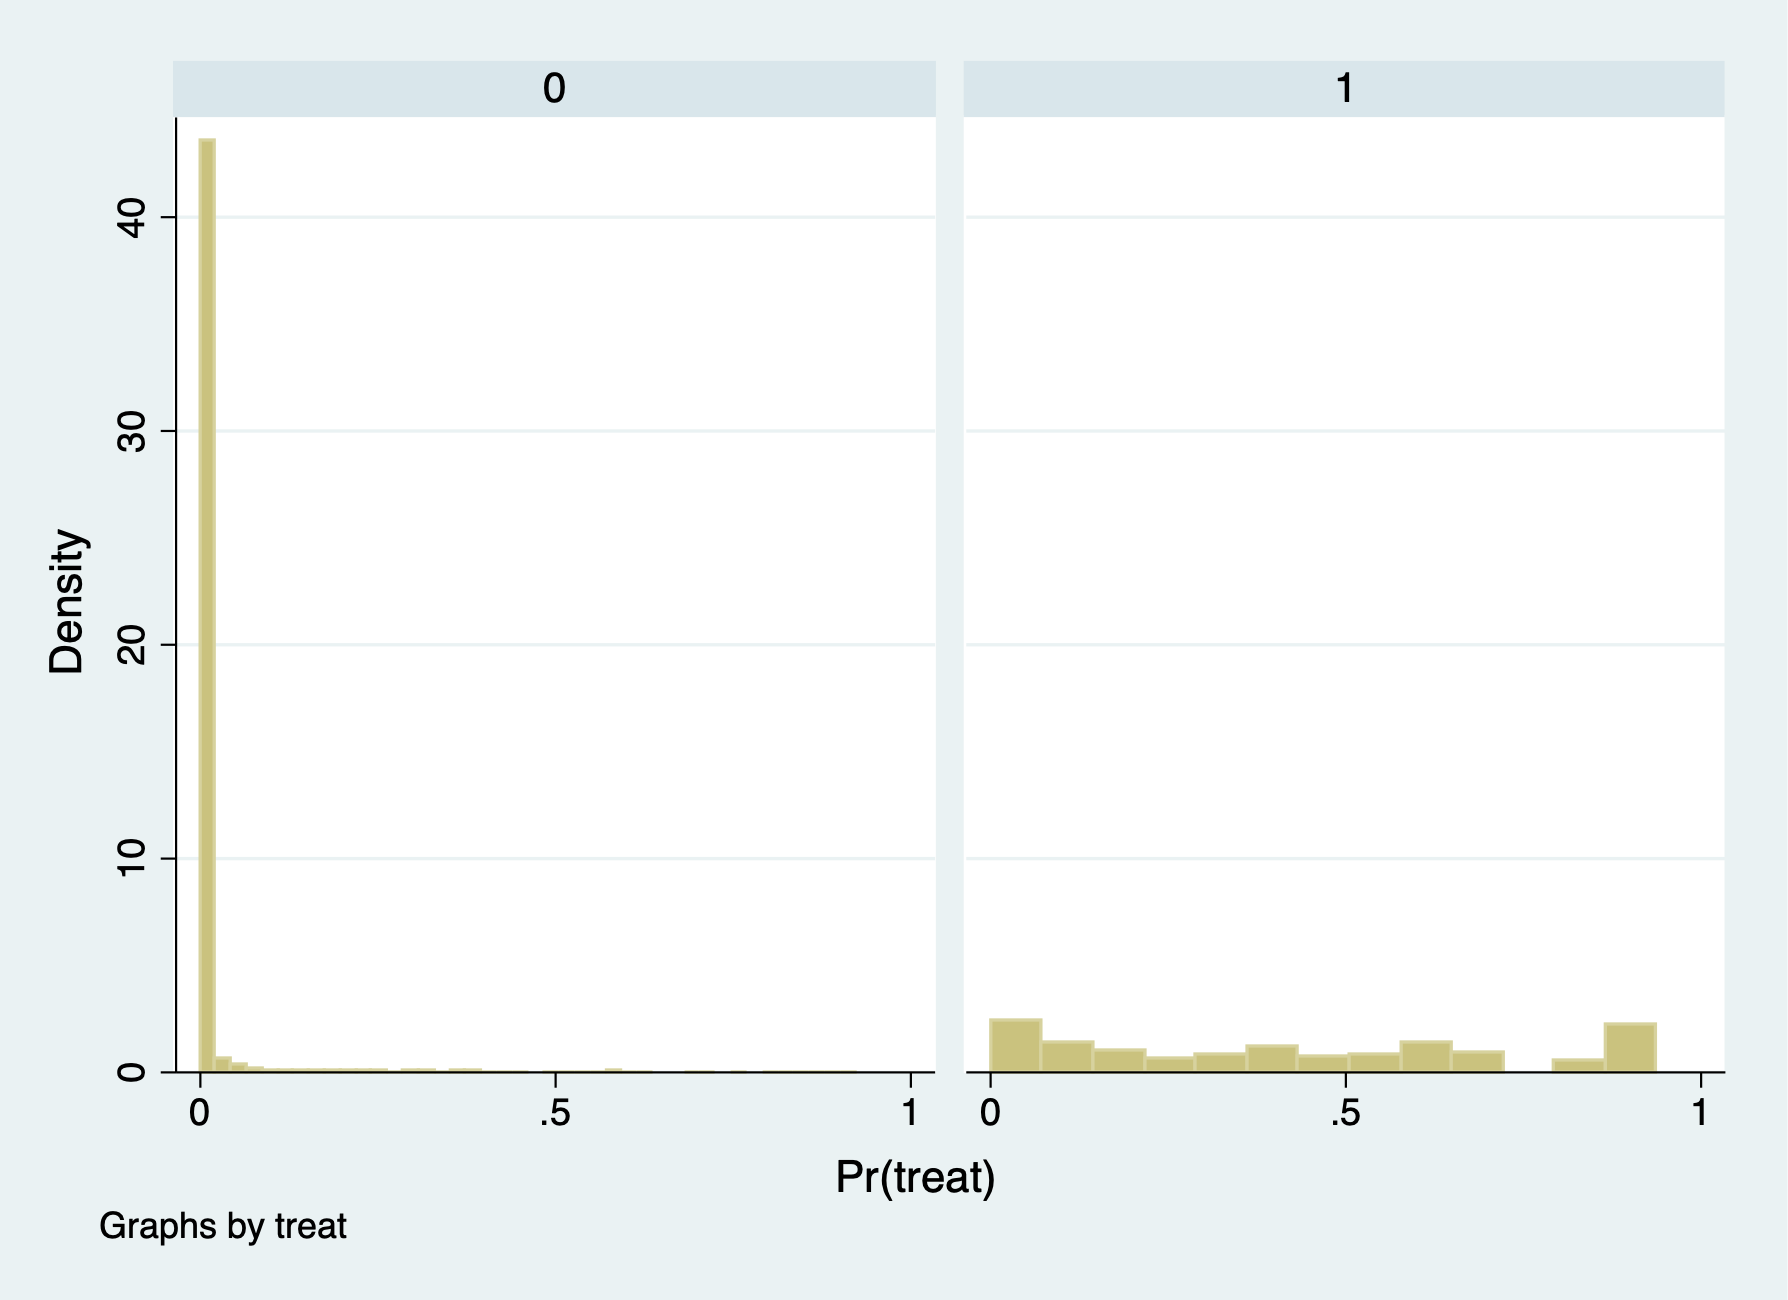
\includegraphics[keepaspectratio]{pscore1.png}}
It seems that there is very little overlap for the common support assumption. It would be problematic to estimate the \(ATE\) and \(ATT\) without trimming to get common support.

\section{\texorpdfstring{Estimate the \(ATE\) and \(ATT\) without trimming}{Estimate the ATE and ATT without trimming}}\label{estimate-the-ate-and-att-without-trimming}

We will estimate the \(ATE\) and \(ATT\) with the \emph{teffects psmatch} command. We will use the 5 nearest neighbors with the option \emph{nn(5)}. Note that Stata generates new variables defined by you. Here we are defining \emph{pstub\_cps}.

Estimate \(ATT\)

\begin{Shaded}
\begin{Highlighting}[]
\NormalTok{teffects psmatch (re78) (treat age agesq agecube educ edusq marr nodegree }\BaseNTok{black} \CommentTok{///}
\NormalTok{ hisp re74 re75 u74 u75 interaction1, }\KeywordTok{logit}\NormalTok{), atet }\KeywordTok{gen}\NormalTok{(pstub\_cps) nn(5)}
\KeywordTok{drop}\NormalTok{ pstub\_cps*}
\end{Highlighting}
\end{Shaded}

\begin{verbatim}
Treatment-effects estimation                   Number of obs      =     16,177
Estimator      : propensity-score matching     Matches: requested =          5
Outcome model  : matching                                     min =          5
Treatment model: logit                                        max =         26
------------------------------------------------------------------------------
             |              AI Robust
        re78 |      Coef.   Std. Err.      z    P>|z|     [95% Conf. Interval]
-------------+----------------------------------------------------------------
ATET         |
       treat |
   (1 vs 0)  |   1725.082   700.0586     2.46   0.014     352.9921    3097.172
------------------------------------------------------------------------------
\end{verbatim}

\(\widehat{ATT} = \$1,725.082\)

We have a few more options for checking the balance after the PSM with nearest neighbor of 5. We can use the \emph{teblance} commands to check our balance. \emph{tebalance density} will give us a distribution of propensity scores by our variable of choice between treatment and comparison. We can also use \emph{tebalance box} that will give is a box-and-whisker chart for the propensity scores by our variable of choice between treatment and comparison.

\begin{Shaded}
\begin{Highlighting}[]
\NormalTok{tebalance }\KeywordTok{summarize}\NormalTok{, baseline}
\end{Highlighting}
\end{Shaded}

\begin{verbatim}
  Covariate balance summary
                                                   Raw      Matched
                          -----------------------------------------
                          Number of obs =       16,177          370
                          Treated obs   =          185          185
                          Control obs   =       15,992          185
                          -----------------------------------------

  -----------------------------------------------------------------
                  |           Means                  Variances     
                  |    Control     Treated       Control    Treated
  ----------------+------------------------------------------------
              age |   33.22524    25.81622      121.9968    51.1943
            agesq |   1225.906    717.3946      615814.1     185978
          agecube |   49305.85    21554.66      2.04e+09   4.40e+08
             educ |   12.02751    10.34595      8.241754   4.042714
            edusq |   152.9023    111.0595      4511.316   1544.795
             marr |   .7117309    .1891892      .2051829   .1542303
         nodegree |   .2958354    .7081081      .2083299   .2078143
            black |   .0735368    .8432432      .0681334   .1329025
             hisp |    .072036    .0594595       .066851    .056228
             re74 |    14016.8    2095.574      9.16e+07   2.39e+07
             re75 |    13650.8    1532.055      8.59e+07   1.04e+07
              u74 |   .1196223    .7081081      .1053194   .2078143
              u75 |   .1093047          .6      .0973632   .2413043
     interaction1 |   171147.6    22898.73      1.67e+10   3.29e+09
  -----------------------------------------------------------------
\end{verbatim}

After running \emph{tebalance summarize}, we can see without trimming that our covariates are not really balanced between treatment and comparison groups.

\begin{Shaded}
\begin{Highlighting}[]
\NormalTok{tebalance density age}
\end{Highlighting}
\end{Shaded}

\begin{figure}
\centering
\pandocbounded{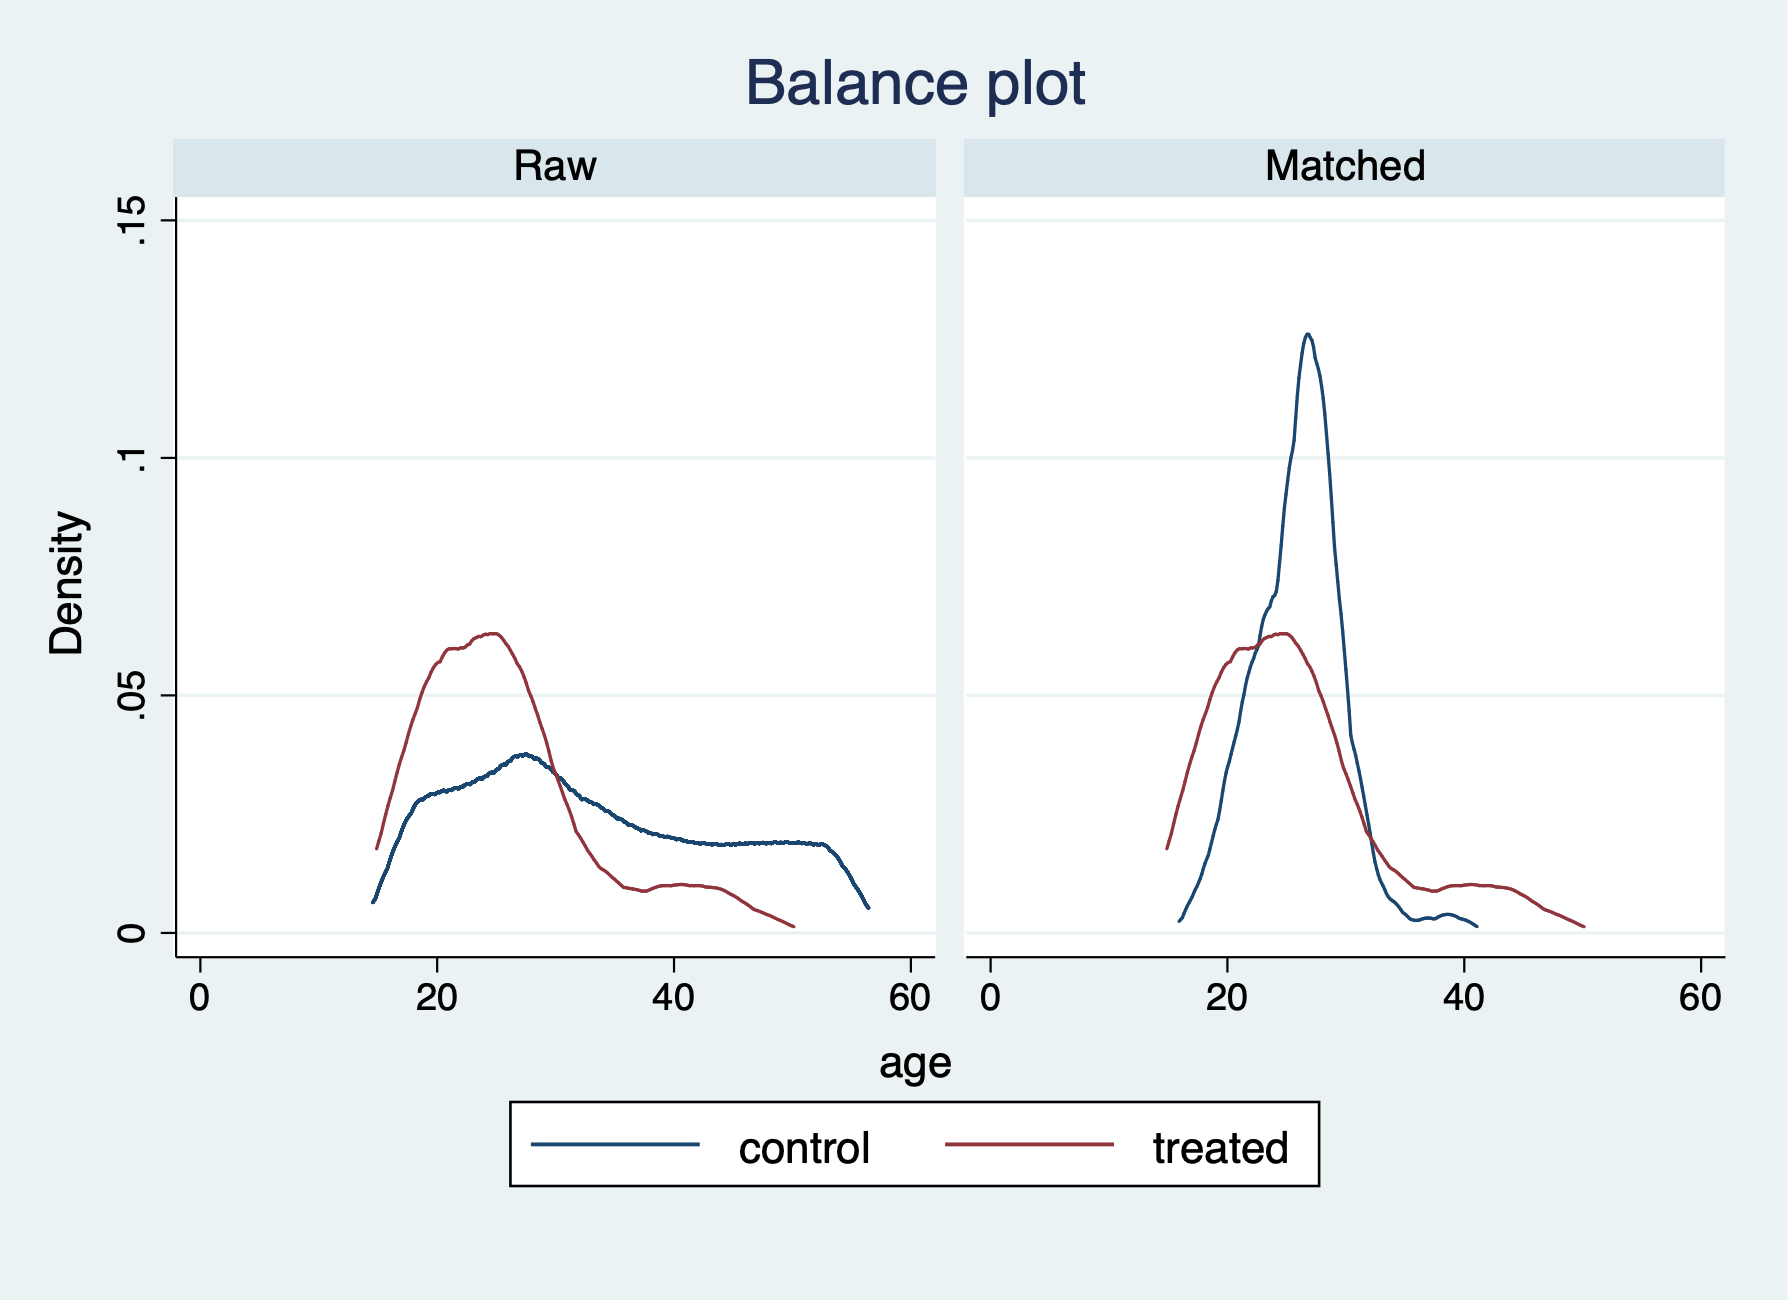
\includegraphics[keepaspectratio]{tebalance_age_1.png}}
\caption{Density Chart for Age}
\end{figure}

\begin{Shaded}
\begin{Highlighting}[]
\NormalTok{tebalance box age}
\KeywordTok{drop}\NormalTok{ pstub\_cps* }
\end{Highlighting}
\end{Shaded}

\begin{figure}
\centering
\pandocbounded{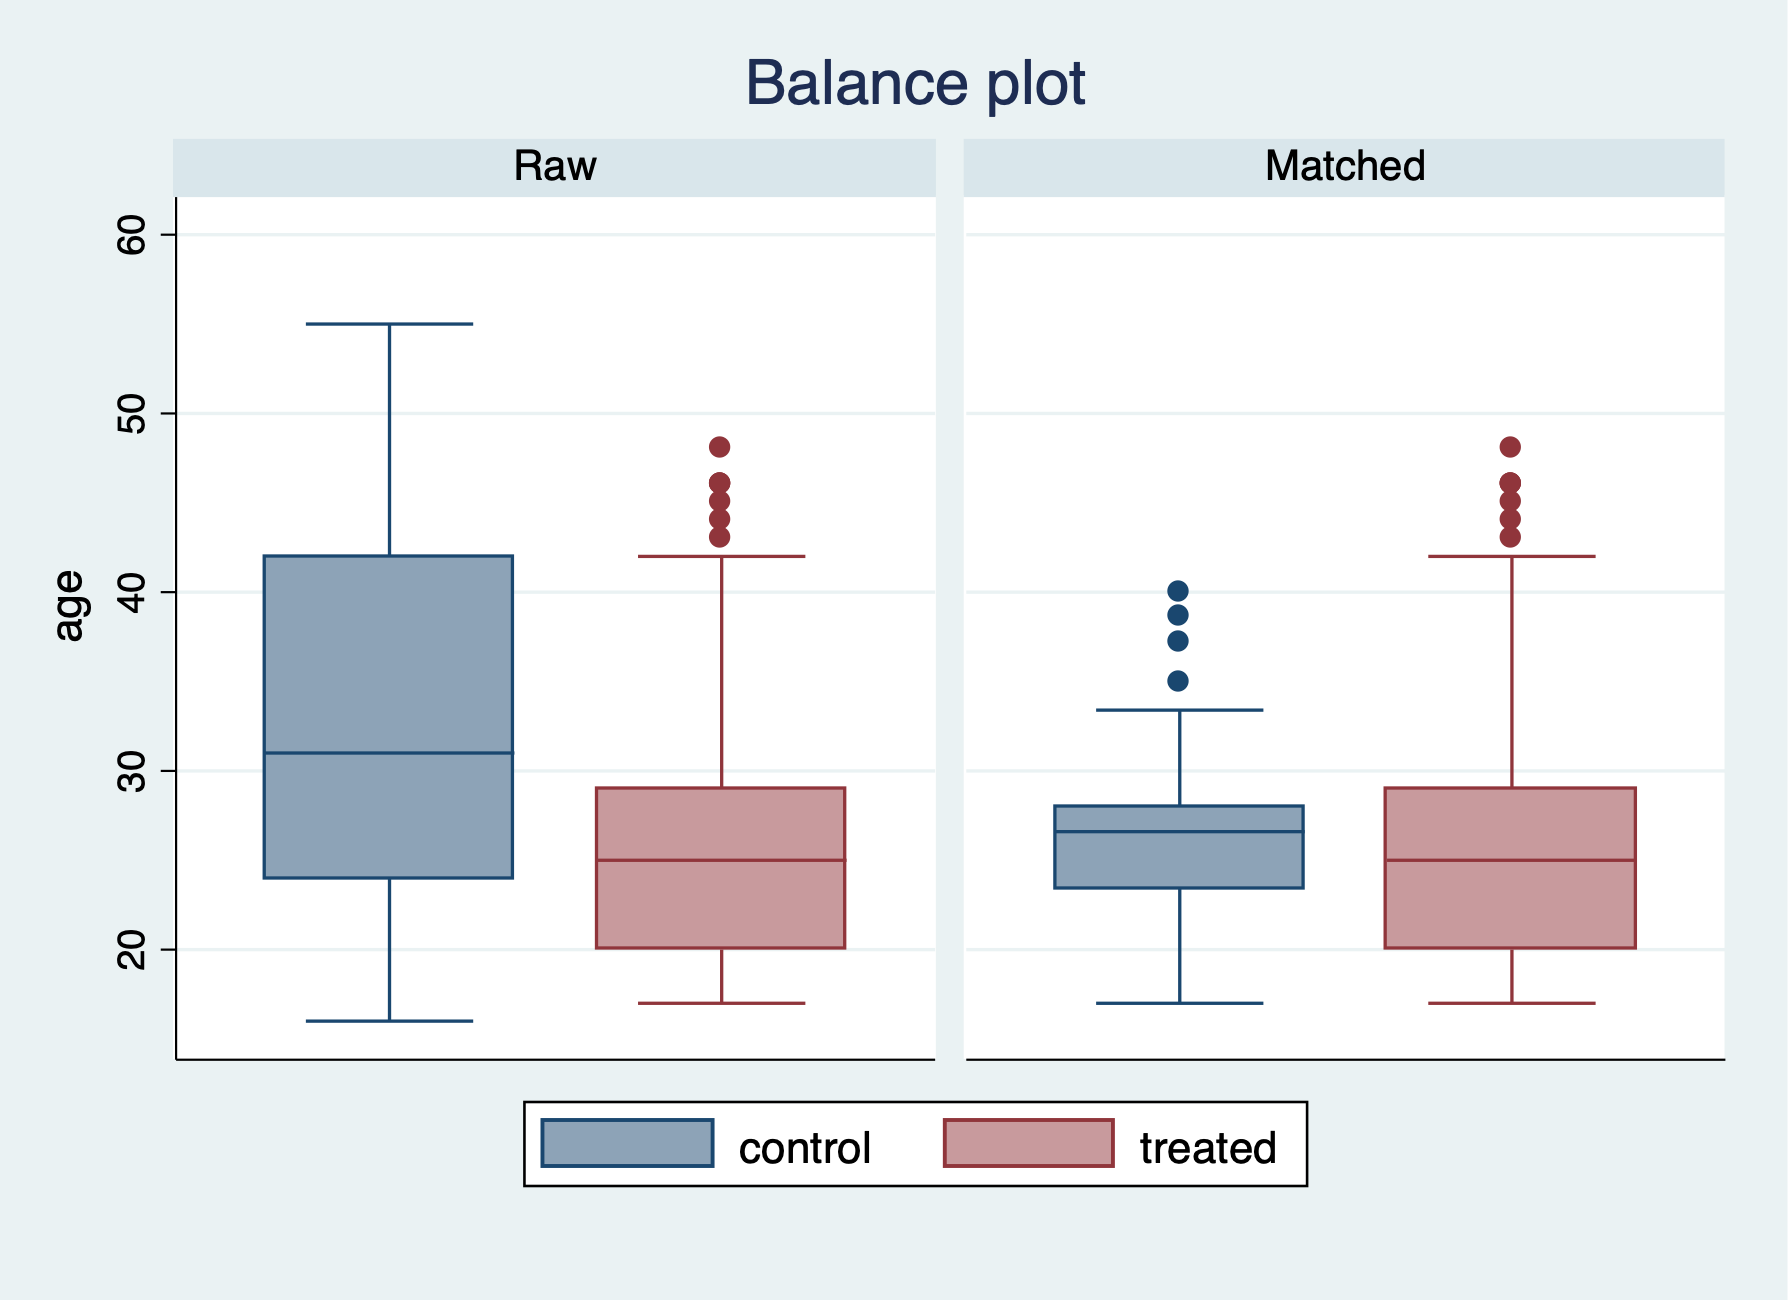
\includegraphics[keepaspectratio]{tebalance_box_1.png}}
\caption{Box Chart for Age}
\end{figure}

Next, we will estimate the \(ATE\) with \emph{teffects psmatch}.

\begin{Shaded}
\begin{Highlighting}[]
\NormalTok{teffects psmatch (re78) (treat age agesq agecube educ edusq marr nodegree }\BaseNTok{black} \CommentTok{///}
\NormalTok{ hisp re74 re75 u74 u75 interaction1, }\KeywordTok{logit}\NormalTok{), ate }\KeywordTok{gen}\NormalTok{(pstub\_cps) nn(5)}

\KeywordTok{drop}\NormalTok{ pstub\_cps*}
\end{Highlighting}
\end{Shaded}

We find that we have an error estimating the \(ATE\), since we lack common support.

\section{Trim the data}\label{trim-the-data}

We will use the trim the \(p\)-scores. All values below \(10\%\) and above \(90\%\) will be dropped.

\begin{Shaded}
\begin{Highlighting}[]
\KeywordTok{drop} \KeywordTok{if}\NormalTok{ pscore \textless{}= 0.1 }
\KeywordTok{drop} \KeywordTok{if}\NormalTok{ pscore \textgreater{}= 0.9}
\end{Highlighting}
\end{Shaded}

We can see that the comparison group has a lot of observations with \(p\)-scores less than or equal to 0.1 (15,802), but we only drop 14 observations with \(p\)-scores greater than or equal 0.9.

\begin{verbatim}
(15,802 observations deleted)

(14 observations deleted)
\end{verbatim}

\section{Check for balance again}\label{check-for-balance-again}

\begin{Shaded}
\begin{Highlighting}[]
\KeywordTok{histogram}\NormalTok{ pscore, }\KeywordTok{by}\NormalTok{(treat) binrescale}
\KeywordTok{graph} \KeywordTok{export} \StringTok{"pscore2.png"}\NormalTok{, }\KeywordTok{replace}
\end{Highlighting}
\end{Shaded}

\pandocbounded{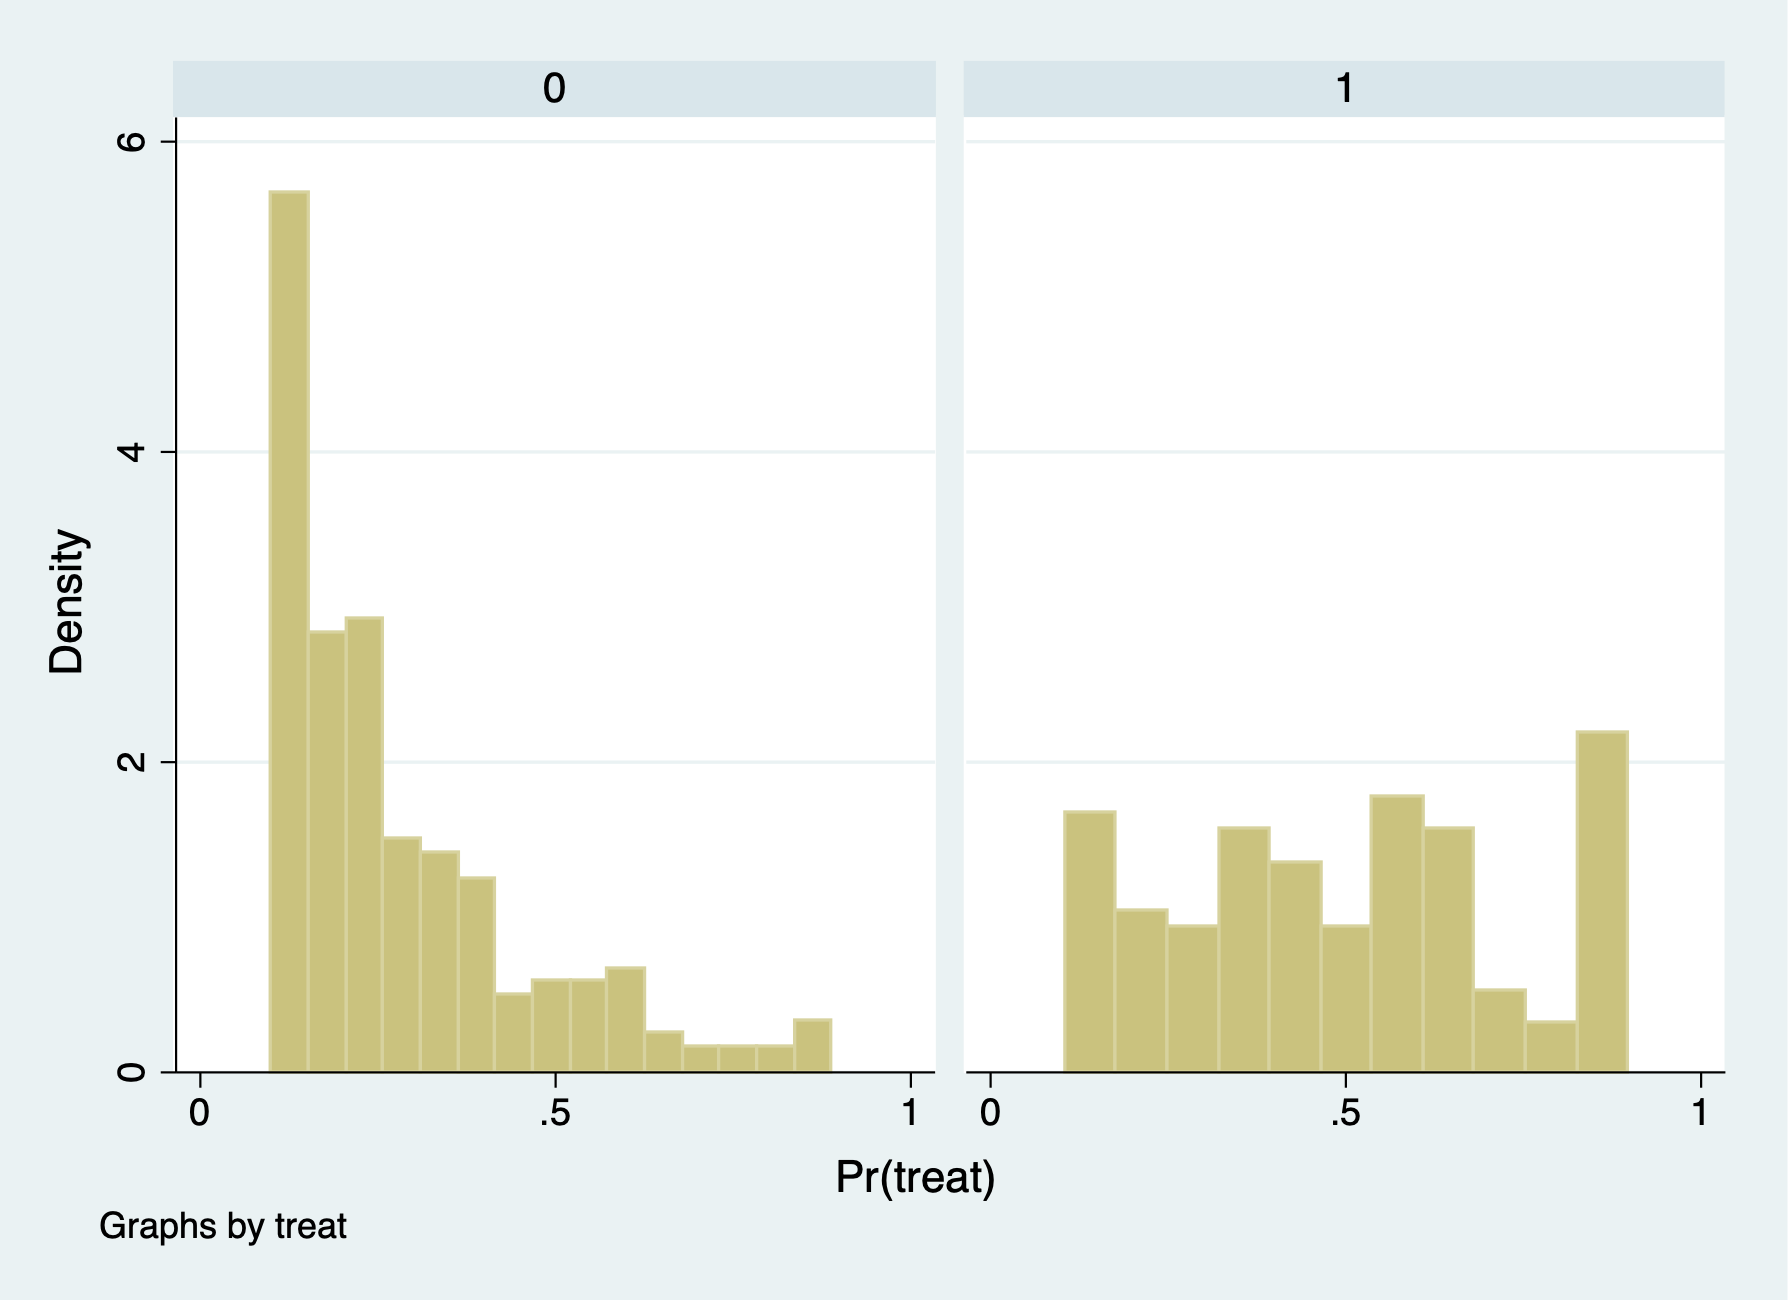
\includegraphics[keepaspectratio]{pscore2.png}}
We can now see we have better overlap between treatment and comparison after trimming the extreme values of the \(p\)-scores.

\section{\texorpdfstring{Reestimate the \(ATT\) and \(ATE\)}{Reestimate the ATT and ATE}}\label{reestimate-the-att-and-ate}

\begin{Shaded}
\begin{Highlighting}[]
\NormalTok{teffects psmatch (re78) (treat age agesq agecube educ edusq marr nodegree }\BaseNTok{black} \CommentTok{///}
\NormalTok{ hisp re74 re75 u74 u75 interaction1, }\KeywordTok{logit}\NormalTok{), ate }\KeywordTok{gen}\NormalTok{(pstub\_cps) nn(5)}

\KeywordTok{drop}\NormalTok{ pstub\_cps*}
\end{Highlighting}
\end{Shaded}

\begin{verbatim}
Treatment-effects estimation                   Number of obs      =        361
Estimator      : propensity-score matching     Matches: requested =          5
Outcome model  : matching                                     min =          5
Treatment model: logit                                        max =          8
------------------------------------------------------------------------------
             |              AI Robust
        re78 |      Coef.   Std. Err.      z    P>|z|     [95% Conf. Interval]
-------------+----------------------------------------------------------------
ATE          |
       treat |
   (1 vs 0)  |   1758.837   724.5845     2.43   0.015     338.6778    3178.997
------------------------------------------------------------------------------
\end{verbatim}

\(\widehat{ATE}= \$1758.84\)

\begin{Shaded}
\begin{Highlighting}[]
\NormalTok{teffects psmatch (re78) (treat age agesq agecube educ edusq marr nodegree }\BaseNTok{black} \CommentTok{///}
\NormalTok{ hisp re74 re75 u74 u75 interaction1, }\KeywordTok{logit}\NormalTok{), atet }\KeywordTok{gen}\NormalTok{(pstub\_cps) nn(5)}
\end{Highlighting}
\end{Shaded}

\begin{verbatim}
Treatment-effects estimation                   Number of obs      =        361
Estimator      : propensity-score matching     Matches: requested =          5
Outcome model  : matching                                     min =          5
Treatment model: logit                                        max =          8
------------------------------------------------------------------------------
             |              AI Robust
        re78 |      Coef.   Std. Err.      z    P>|z|     [95% Conf. Interval]
-------------+----------------------------------------------------------------
ATET         |
       treat |
   (1 vs 0)  |   2519.446   866.7552     2.91   0.004     820.6375    4218.255
------------------------------------------------------------------------------
\end{verbatim}

\(\widehat{ATE}= \$2519.446\)

\section{Recheck for balance}\label{recheck-for-balance}

\begin{Shaded}
\begin{Highlighting}[]
\NormalTok{tebalance }\KeywordTok{summarize}\NormalTok{, baseline}
\end{Highlighting}
\end{Shaded}

\begin{verbatim}
  Covariate balance summary
                                                   Raw      Matched
                          -----------------------------------------
                          Number of obs =          361          266
                          Treated obs   =          133          133
                          Control obs   =          228          133
                          -----------------------------------------

  -----------------------------------------------------------------
                  |           Means                  Variances     
                  |    Control     Treated       Control    Treated
  ----------------+------------------------------------------------
              age |   25.93421     25.2406      64.98684   45.00228
            agesq |   737.2851    681.7519        237422   158499.2
          agecube |   22966.88    19825.29      6.03e+08   3.66e+08
             educ |   10.46491     10.2406      4.584667   3.850763
            edusq |   114.0789    108.6917      1830.681   1331.306
             marr |   .2192982    .1428571      .1719607   .1233766
         nodegree |   .6315789    .7518797       .233712   .1879699
            black |   .9342105    .9398496       .061732   .0569606
             hisp |   .0438596     .037594      .0421207   .0364548
             re74 |   2552.555    1560.604      1.93e+07   1.56e+07
             re75 |   1570.309    1002.193       7324536    3233917
              u74 |   .5570175    .7669173       .247836   .1801094
              u75 |   .4868421    .6390977      .2509274   .2323992
     interaction1 |   27361.94    16425.15      2.44e+09   1.81e+09
  -----------------------------------------------------------------
\end{verbatim}

Our balance is greatly improved after trimming the tail ends of the propensity scores.

Let's check the variable age with \emph{tebalance density} and \emph{tebalance box}.

\begin{Shaded}
\begin{Highlighting}[]
\NormalTok{tebalance density age}
\end{Highlighting}
\end{Shaded}

\begin{figure}
\centering
\pandocbounded{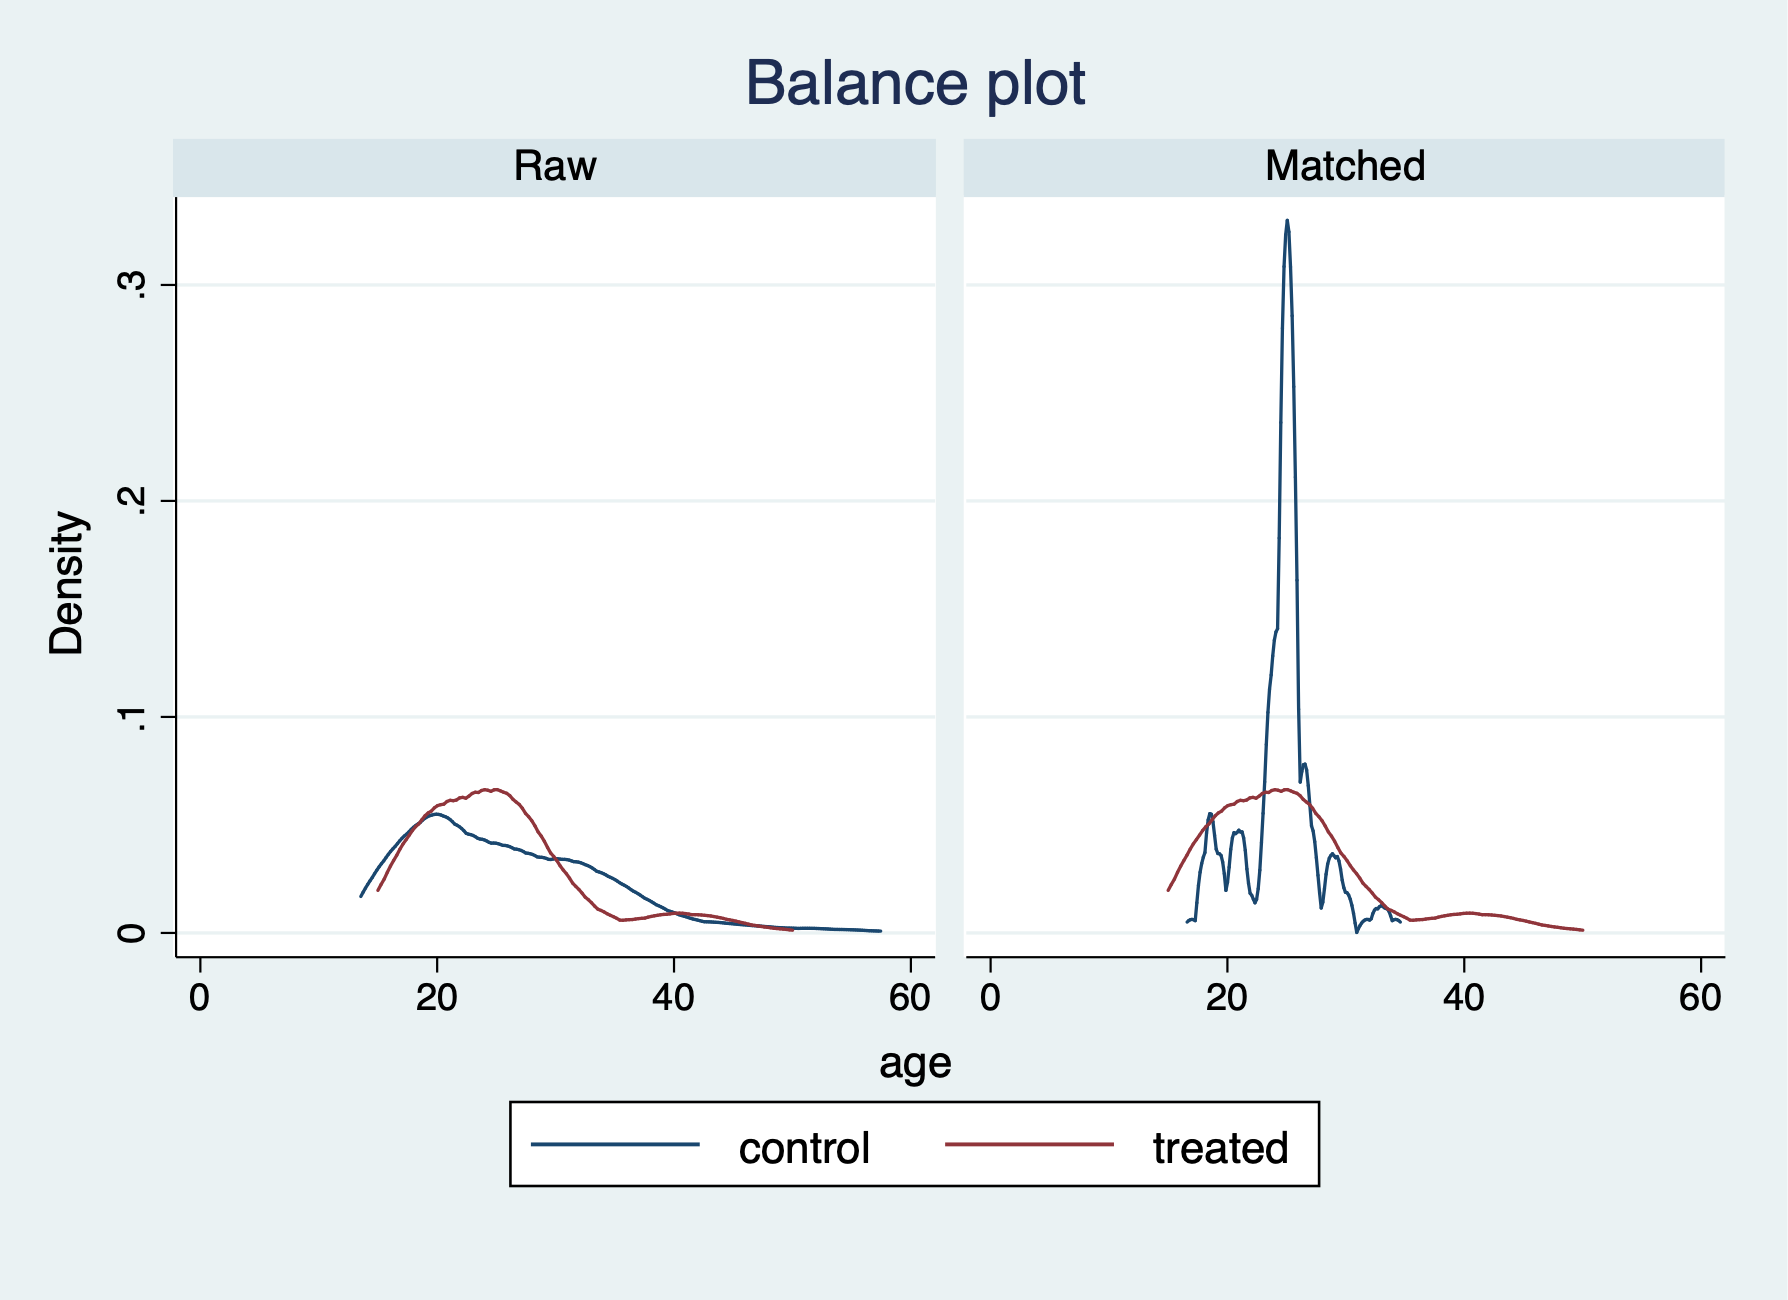
\includegraphics[keepaspectratio]{tebalance_age_2.png}}
\caption{Density Chart of Age After Trimming}
\end{figure}

\begin{Shaded}
\begin{Highlighting}[]
\NormalTok{tebalance box age}
\end{Highlighting}
\end{Shaded}

\begin{figure}
\centering
\pandocbounded{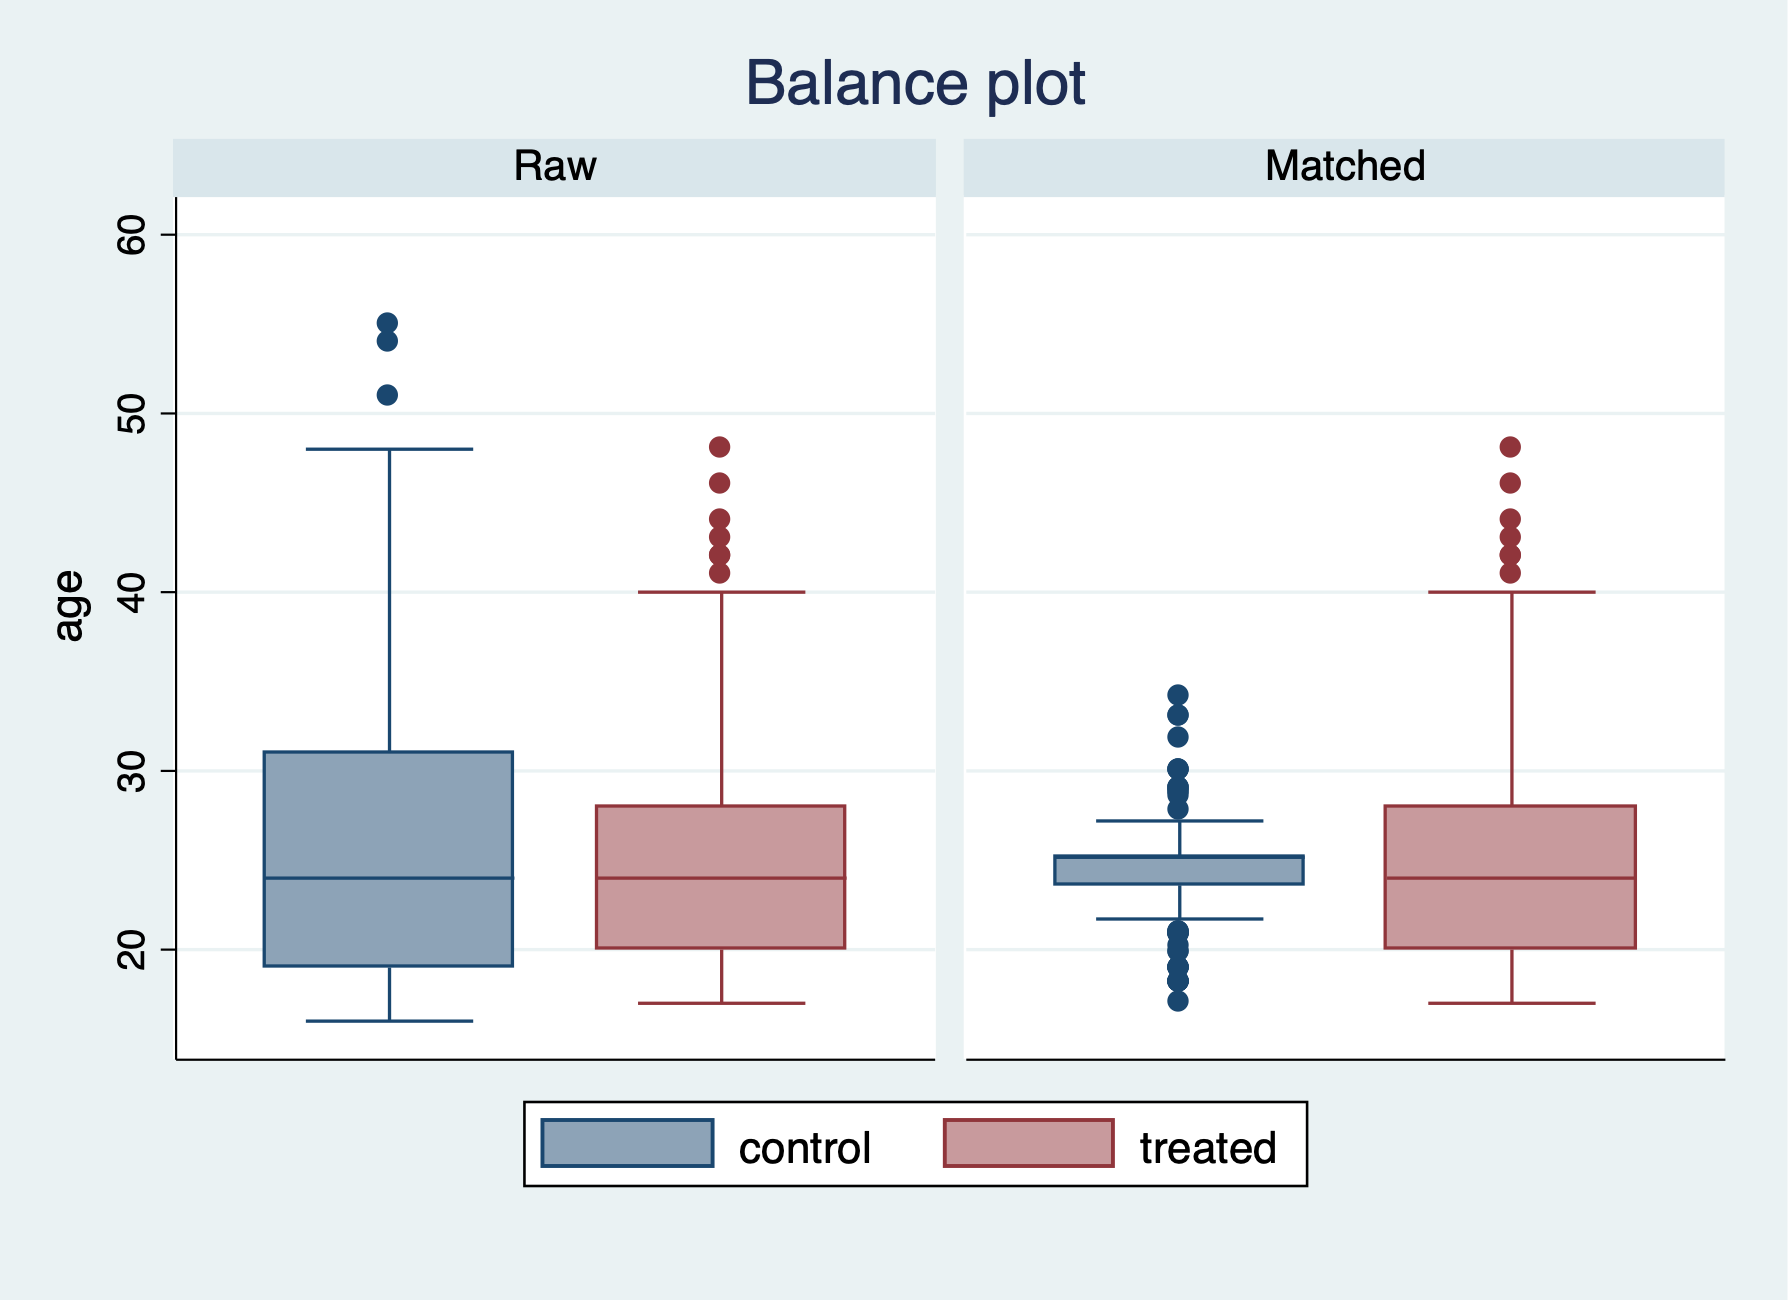
\includegraphics[keepaspectratio]{tebalance_box_2.png}}
\caption{Box Chart of Age After Trimming}
\end{figure}

\chapter{Inverse Probability Weights}\label{inverse-probability-weights}

We will reload our treatment group and CPS comparison group, and use the \emph{teffects ipw} command to estimate the \(ATE\).

We will repull our data, estimate our \(p\)-score, and check our balance

\begin{Shaded}
\begin{Highlighting}[]
\NormalTok{*Get Data}
\KeywordTok{use}\NormalTok{ https:}\CommentTok{//github.com/scunning1975/mixtape/raw/master/nsw\_mixtape.dta, clear}
\KeywordTok{drop} \KeywordTok{if}\NormalTok{ treat==0}
\KeywordTok{append} \KeywordTok{using}\NormalTok{ https:}\CommentTok{//github.com/scunning1975/mixtape/raw/master/cps\_mixtape.dta}

\NormalTok{*Calculate Variables}
\KeywordTok{gen}\NormalTok{ agesq=age*age}
\KeywordTok{gen}\NormalTok{ agecube=age*age*age}
\KeywordTok{gen}\NormalTok{ edusq=educ*edu}
\KeywordTok{gen}\NormalTok{ u74 = 0 }\KeywordTok{if}\NormalTok{ re74!=.}
\KeywordTok{replace}\NormalTok{ u74 = 1 }\KeywordTok{if}\NormalTok{ re74==0}
\KeywordTok{gen}\NormalTok{ u75 = 0 }\KeywordTok{if}\NormalTok{ re75!=.}
\KeywordTok{replace}\NormalTok{ u75 = 1 }\KeywordTok{if}\NormalTok{ re75==0}
\KeywordTok{gen}\NormalTok{ interaction1 = educ*re74}
\KeywordTok{gen}\NormalTok{ re74sq=re74\^{}2}
\KeywordTok{gen}\NormalTok{ re75sq=re75\^{}2}
\KeywordTok{gen}\NormalTok{ interaction2 = u74*hisp}

\NormalTok{*Estimate the coefficients}
\KeywordTok{logit}\NormalTok{ treat age agesq agecube educ edusq marr nodegree }\BaseNTok{black}\NormalTok{ hisp re74 re75 u74 u75 interaction1 }
\KeywordTok{predict}\NormalTok{ pscore}

\NormalTok{* Checking }\KeywordTok{mean}\NormalTok{ propensity scores }\KeywordTok{for}\NormalTok{ treatment and control groups}
\KeywordTok{sum}\NormalTok{ pscore }\KeywordTok{if}\NormalTok{ treat==1, }\KeywordTok{detail}
\KeywordTok{sum}\NormalTok{ pscore }\KeywordTok{if}\NormalTok{ treat==0, }\KeywordTok{detail}

\NormalTok{* Now look }\FunctionTok{at}\NormalTok{ the propensity }\KeywordTok{score}\NormalTok{ distribution }\KeywordTok{for}\NormalTok{ treatment and control groups}
\KeywordTok{histogram}\NormalTok{ pscore, }\KeywordTok{by}\NormalTok{(treat) binrescale}
\end{Highlighting}
\end{Shaded}

\begin{figure}
\centering
\pandocbounded{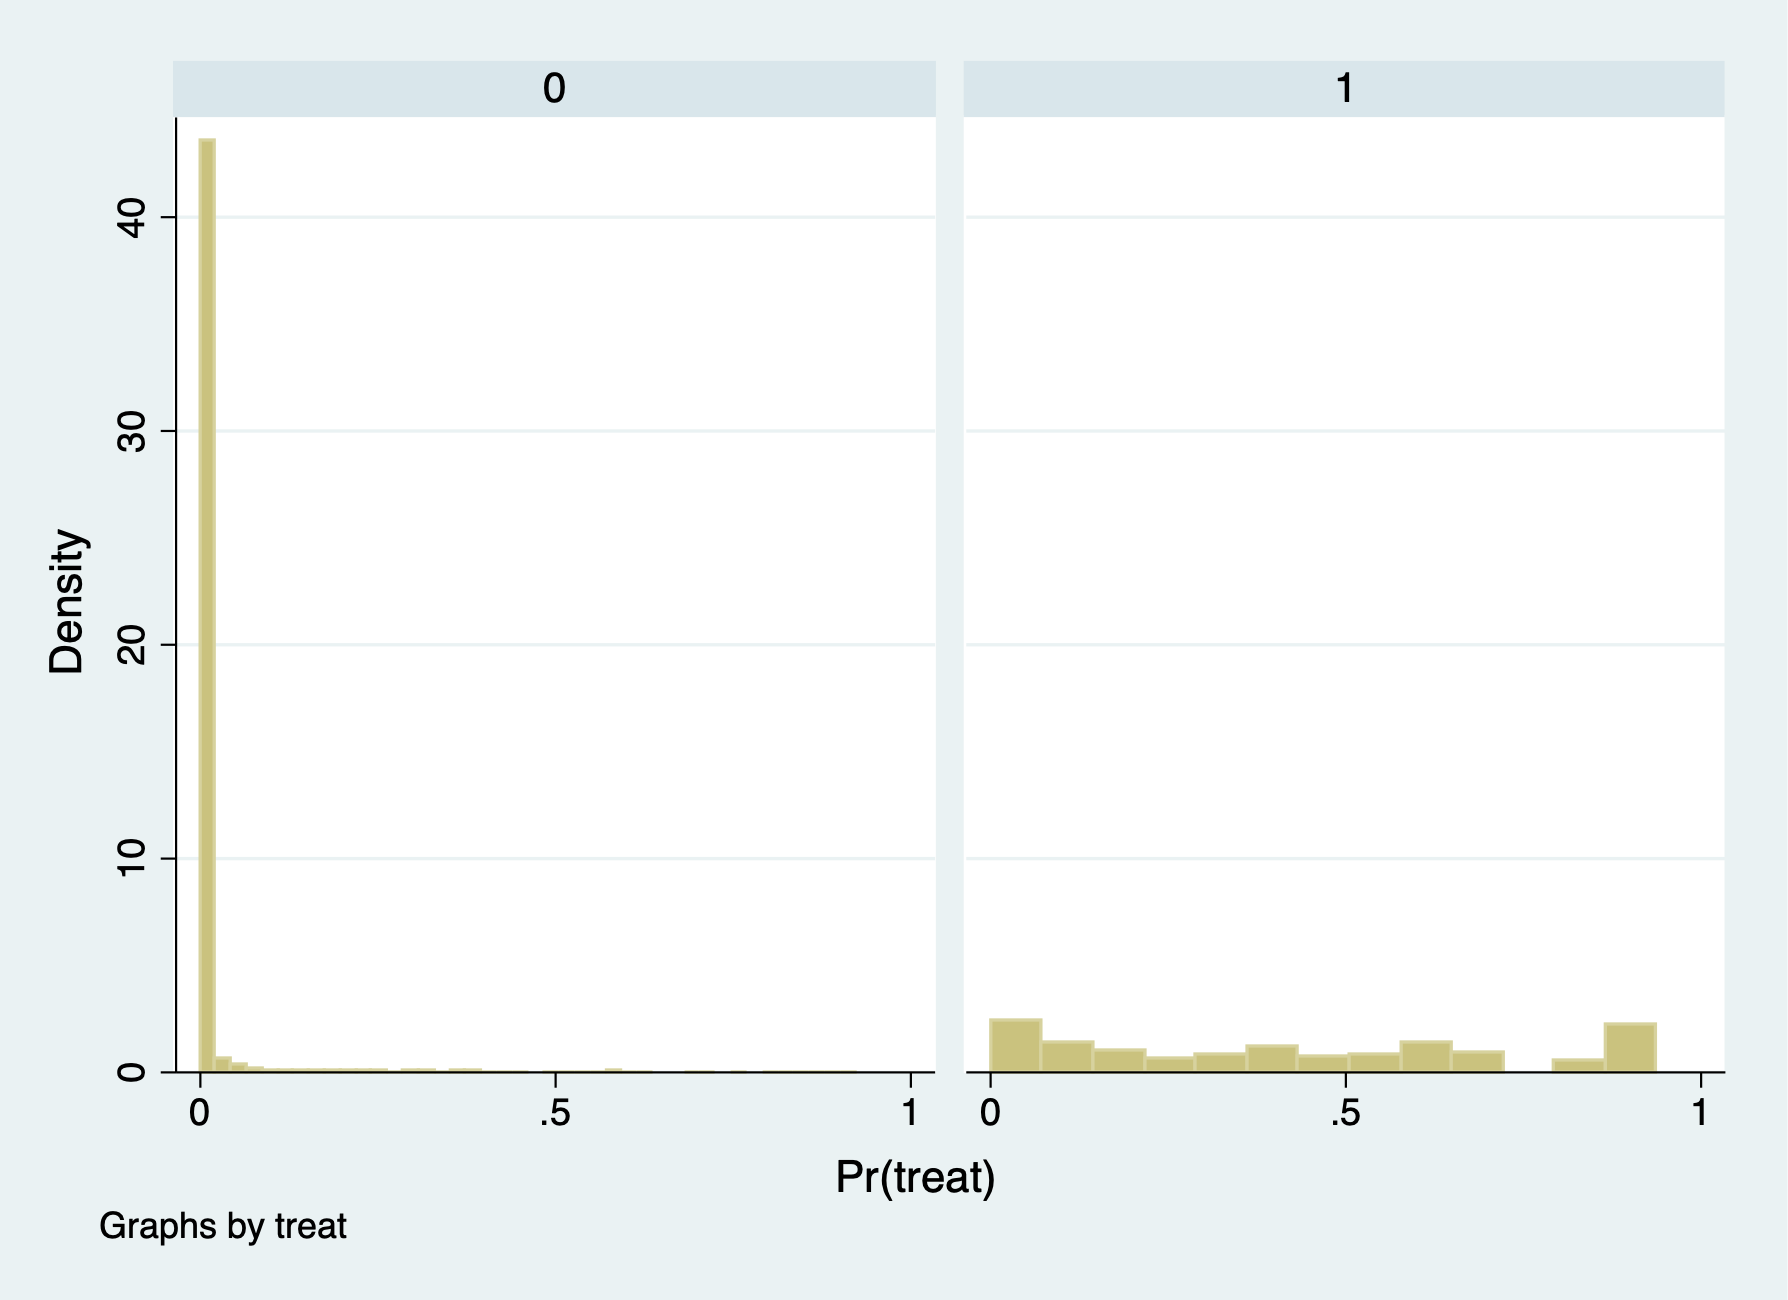
\includegraphics[keepaspectratio]{pscore1.png}}
\caption{Histogram for IPW}
\end{figure}

\section{\texorpdfstring{Manual Calculate the \(ATE\)}{Manual Calculate the ATE}}\label{manual-calculate-the-ate}

We will manually calculate inverse probability weighting (IPW) with Propensity Scores. Please note that IPW is not matching, even though we use propensity scores.

\textbf{IPW with Non-normalized Weights:}
\[ \widehat{ATE} = \frac{1}{n}*\sum_{n=1}^{N} \left( {\frac{Y_i*D_i}{\hat{p}(x)_i}} \right)-\frac{1}{n}*\sum_{n=1}^{N} \left( {\frac{Y_i*(1-D_i)}{1-\hat{p}(x)_i}} \right) \]

\textbf{IPW with Normalized Weights:}

\[ \widehat{ATE}=\left[\sum_{n=1}^{N}\frac{Y_i*D_i}{\hat{p}(x)_i} \right] / \left[\sum_{n=1}^{N}\frac{D_i}{\hat{p}(x)_i} \right] - \left[\sum_{n=1}^{N}\frac{Y_i*(1-D_i)}{(1-\hat{p}(x)_i)} \right] / \left[\sum_{n=1}^{N}\frac{(1-D_i)}{(1-\hat{p}(x)_i)} \right] \]

\subsection{\texorpdfstring{Calculate \(E[Y^1]\) and \(E[Y^0]\)}{Calculate E{[}Y\^{}1{]} and E{[}Y\^{}0{]}}}\label{calculate-ey1-and-ey0}

First, we need to calculate normalization weights

\begin{Shaded}
\begin{Highlighting}[]
\KeywordTok{gen}\NormalTok{ d1=treat/pscore}
\KeywordTok{gen} \KeywordTok{d0}\NormalTok{=(1{-}treat)/(1{-}pscore)}
\end{Highlighting}
\end{Shaded}

Sum the inverse pscore

\begin{Shaded}
\begin{Highlighting}[]
\KeywordTok{egen}\NormalTok{ s1=}\KeywordTok{sum}\NormalTok{(d1)}
\KeywordTok{egen}\NormalTok{ s0=}\KeywordTok{sum}\NormalTok{(}\KeywordTok{d0}\NormalTok{) }
\KeywordTok{gen} \KeywordTok{total}\NormalTok{ = \_N}
\KeywordTok{egen}\NormalTok{ total\_T = }\KeywordTok{sum}\NormalTok{(treat)}
\KeywordTok{egen}\NormalTok{ total\_C = }\KeywordTok{sum}\NormalTok{(1{-}treat)}
\end{Highlighting}
\end{Shaded}

First, we will manually calculate \(E[Y^1]\) with non-normalized weights using all the data. Calculate \(E[Y^1]=\frac{1}{n}*\sum_{n=1}^{N}\frac{Y_i*D_i}{\hat{p}(x)_i}\)

\begin{Shaded}
\begin{Highlighting}[]
\KeywordTok{gen}\NormalTok{ y1=treat*re78/pscore}
\KeywordTok{egen}\NormalTok{ y1\_2 = }\KeywordTok{sum}\NormalTok{(y1)}
\KeywordTok{gen}\NormalTok{ y1\_3 = y1\_2/}\KeywordTok{total}
\end{Highlighting}
\end{Shaded}

Next, we will manually calculate \(E[Y^0]\) with non-normalized weights using all the data. Calculate \(E[Y^0]=\frac{1}{n}*\sum_{n=1}^{N}\frac{Y*(1-D_i)}{(1-\hat{p}(x)_i)}\)

\begin{Shaded}
\begin{Highlighting}[]
\KeywordTok{gen}\NormalTok{ y0=(1{-}treat)*re78/(1{-}pscore) }
\KeywordTok{egen}\NormalTok{ y0\_2 = }\KeywordTok{sum}\NormalTok{(y0)}
\KeywordTok{gen}\NormalTok{ y0\_3 = y0\_2/}\KeywordTok{total}
\end{Highlighting}
\end{Shaded}

Then calculate the \(ATE\) by taking the difference in \(E[Y^1]-E[Y^0]\).

\begin{Shaded}
\begin{Highlighting}[]
\NormalTok{*Way 1}
\KeywordTok{gen}\NormalTok{ ht=y1{-}y0}
\NormalTok{*Way 2}
\KeywordTok{gen}\NormalTok{ ht2=y1\_3{-}y0\_3}
\NormalTok{*Same results}
\KeywordTok{sum}\NormalTok{ ht ht2}
\end{Highlighting}
\end{Shaded}

\begin{verbatim}
    Variable |        Obs        Mean    Std. Dev.       Min        Max
-------------+---------------------------------------------------------
          ht |     16,177   -11876.79    127578.8  -99232.64   1.19e+07
         ht2 |     16,177   -11876.79           0  -11876.79  -11876.79
\end{verbatim}

Now we will calculate the \(ATE\) manually using normalized weights

\begin{Shaded}
\begin{Highlighting}[]
\NormalTok{*Way 1}
\KeywordTok{replace}\NormalTok{ y1=(treat*re78/pscore)/(s1/}\KeywordTok{total}\NormalTok{)}
\KeywordTok{replace}\NormalTok{ y0=((1{-}treat)*re78/(1{-}pscore))/(s0/}\KeywordTok{total}\NormalTok{)}
\NormalTok{*Way 2}
\KeywordTok{replace}\NormalTok{ y1\_3=y1\_2/s1}
\KeywordTok{replace}\NormalTok{ y0\_3=y0\_2/s0}
\NormalTok{*Get the estimated ATE}
\KeywordTok{gen} \FunctionTok{norm}\NormalTok{=y1{-}y0}
\KeywordTok{gen}\NormalTok{ norm2=y1\_3{-}y0\_3}
\NormalTok{*Same Results }\KeywordTok{for}\NormalTok{ ht:ht2 and }\FunctionTok{norm}\NormalTok{:norm2}
\KeywordTok{sum}\NormalTok{ ht ht2 }\FunctionTok{norm}\NormalTok{ norm2}
\end{Highlighting}
\end{Shaded}

\begin{verbatim}
(140 real changes made)

(13,820 real changes made)

(16,177 real changes made)

(16,177 real changes made)

    Variable |        Obs        Mean    Std. Dev.       Min        Max
-------------+---------------------------------------------------------
          ht |     16,177   -11876.79    127578.8  -99232.64   1.19e+07
         ht2 |     16,177   -11876.79           0  -11876.79  -11876.79
        norm |     16,177    -7238.14    332633.6   -99127.2   3.11e+07
       norm2 |     16,177    -7238.14           0   -7238.14   -7238.14
\end{verbatim}

ATE under non-normalized weights is -\$11,876.
ATE under normalized weights is -\$7,238.

Why are they so much different than the experimental research design estimates? Given that the mean \(1-p(x)\) is close to 1, a lot of weight is given to \(Y^0\). What we need to do is trim and recalculate.

\subsection{Trim the data}\label{trim-the-data-1}

We will drop our calculated variables and then trim our \(p\)-scores.

\begin{Shaded}
\begin{Highlighting}[]
\KeywordTok{drop}\NormalTok{ d1 }\KeywordTok{d0}\NormalTok{ s1 s0 y1 y0 ht }\FunctionTok{norm}
\KeywordTok{drop} \KeywordTok{if}\NormalTok{ pscore \textless{}= 0.1 }
\KeywordTok{drop} \KeywordTok{if}\NormalTok{ pscore \textgreater{}= 0.9}
\end{Highlighting}
\end{Shaded}

We will recalculate the non-normalized weights using trimmed data.

\begin{Shaded}
\begin{Highlighting}[]
\KeywordTok{gen}\NormalTok{ d1=treat/pscore}
\KeywordTok{gen} \KeywordTok{d0}\NormalTok{=(1{-}treat)/(1{-}pscore)}
\KeywordTok{egen}\NormalTok{ s1=}\KeywordTok{sum}\NormalTok{(d1)}
\KeywordTok{egen}\NormalTok{ s0=}\KeywordTok{sum}\NormalTok{(}\KeywordTok{d0}\NormalTok{)}

\KeywordTok{gen}\NormalTok{ y1=treat*re78/pscore}
\KeywordTok{gen}\NormalTok{ y0=(1{-}treat)*re78/(1{-}pscore)}
\KeywordTok{gen}\NormalTok{ ht=y1{-}y0}
\end{Highlighting}
\end{Shaded}

We will recalculate the normalized weights using trimmed data.

\begin{Shaded}
\begin{Highlighting}[]
\KeywordTok{replace}\NormalTok{ y1=(treat*re78/pscore)/(s1/\_N)}
\KeywordTok{replace}\NormalTok{ y0=((1{-}treat)*re78/(1{-}pscore))/(s0/\_N)}
\KeywordTok{gen} \FunctionTok{norm}\NormalTok{=y1{-}y0}
\KeywordTok{sum}\NormalTok{ ht }\FunctionTok{norm}
\end{Highlighting}
\end{Shaded}

\begin{verbatim}
(0 real changes made)

(0 real changes made)

(0 real changes made)

    Variable |        Obs        Mean    Std. Dev.       Min        Max
-------------+---------------------------------------------------------
          ht |        361    2006.365    19656.33  -73545.45   131755.3
        norm |        361     1806.73    18967.72  -72480.23   126251.9
\end{verbatim}

ATE under non-normalized weights is \$2,006, while the estimated ATE under normalized weights is \$1,807.

These are much closer to our experimental research design estimates.

\section{\texorpdfstring{Calculate \(ATE\) and \(ATT\) using \emph{teffects}}{Calculate ATE and ATT using teffects}}\label{calculate-ate-and-att-using-teffects}

Luckily, we have a built-in Stata command with \emph{teffects ipw}, so we don't need to manually calculate the \(ATE\) everytime. (However, it is a good exercise to see how Stata calculate the estimate). The \emph{teffects} command will also calculate our standard errors, as well.

We will reload our data, trim the data, and use the \emph{teffects ipw} command. We will also trim our data, since we know that there is a lack of overlap at the tail ends of the estimated \(p\)-scores.

\begin{Shaded}
\begin{Highlighting}[]
\NormalTok{* Reload Data}
\KeywordTok{use}\NormalTok{ https:}\CommentTok{//github.com/scunning1975/mixtape/raw/master/nsw\_mixtape.dta, clear}
\KeywordTok{drop} \KeywordTok{if}\NormalTok{ treat==0}

\NormalTok{*Now }\KeywordTok{merge} \KeywordTok{in}\NormalTok{ the CPS controls from footnote 2 }\KeywordTok{of}\NormalTok{ Table 2 (Dehejia and Wahba 2002)}
\KeywordTok{append} \KeywordTok{using}\NormalTok{ https:}\CommentTok{//github.com/scunning1975/mixtape/raw/master/cps\_mixtape.dta}
\KeywordTok{gen}\NormalTok{ agesq=age*age}
\KeywordTok{gen}\NormalTok{ agecube=age*age*age}
\KeywordTok{gen}\NormalTok{ edusq=educ*edu}
\KeywordTok{gen}\NormalTok{ u74 = 0 }\KeywordTok{if}\NormalTok{ re74!=.}
\KeywordTok{replace}\NormalTok{ u74 = 1 }\KeywordTok{if}\NormalTok{ re74==0}
\KeywordTok{gen}\NormalTok{ u75 = 0 }\KeywordTok{if}\NormalTok{ re75!=.}
\KeywordTok{replace}\NormalTok{ u75 = 1 }\KeywordTok{if}\NormalTok{ re75==0}
\KeywordTok{gen}\NormalTok{ interaction1 = educ*re74}
\KeywordTok{gen}\NormalTok{ re74sq=re74\^{}2}
\KeywordTok{gen}\NormalTok{ re75sq=re75\^{}2}
\KeywordTok{gen}\NormalTok{ interaction2 = u74*hisp}

\NormalTok{* Now estimate the propensity }\KeywordTok{score}
\KeywordTok{logit}\NormalTok{ treat age agesq agecube educ edusq marr nodegree }\BaseNTok{black}\NormalTok{ hisp re74 re75 u74 u75 interaction1 }
\KeywordTok{predict}\NormalTok{ pscore}

\NormalTok{* Checking }\KeywordTok{mean}\NormalTok{ propensity scores }\KeywordTok{for}\NormalTok{ treatment and control groups}
\KeywordTok{sum}\NormalTok{ pscore }\KeywordTok{if}\NormalTok{ treat==1, }\KeywordTok{detail}
\KeywordTok{sum}\NormalTok{ pscore }\KeywordTok{if}\NormalTok{ treat==0, }\KeywordTok{detail}

\NormalTok{* Trimming the propensity }\KeywordTok{score}
\KeywordTok{drop} \KeywordTok{if}\NormalTok{ pscore \textless{}= 0.1 }
\KeywordTok{drop} \KeywordTok{if}\NormalTok{ pscore \textgreater{}= 0.9}
\end{Highlighting}
\end{Shaded}

With the \emph{teffects} command, we need to specify \emph{ipw} for inverse probability weights and we need to use the option \emph{logit} to tell Stata to calculate the \(p\)-scores using a logistic regresion. In addition, we will use the option \emph{osample} to look for any overlap between treatment and comparison. Finally, we will use the option \emph{atet} to specify that we want to estimate the \(ATT\).

\begin{Shaded}
\begin{Highlighting}[]
\NormalTok{teffects ipw (re78) (treat age agesq agecube educ edusq marr nodegree }\CommentTok{///}
\BaseNTok{black}\NormalTok{ hisp re74 re75 u74 u75 interaction1, }\KeywordTok{logit}\NormalTok{), osample(overlap) atet}
\KeywordTok{capture} \KeywordTok{drop}\NormalTok{ overlap}
\end{Highlighting}
\end{Shaded}

\begin{verbatim}
Iteration 0:   EE criterion =  1.392e-21  
Iteration 1:   EE criterion =  2.898e-23  

Treatment-effects estimation                    Number of obs     =        361
Estimator      : inverse-probability weights
Outcome model  : weighted mean
Treatment model: logit
------------------------------------------------------------------------------
             |               Robust
        re78 |      Coef.   Std. Err.      z    P>|z|     [95% Conf. Interval]
-------------+----------------------------------------------------------------
ATET         |
       treat |
   (1 vs 0)  |   2646.866   892.2393     2.97   0.003     898.1089    4395.623
-------------+----------------------------------------------------------------
POmean       |
       treat |
          0  |   3791.931   514.4727     7.37   0.000     2783.582    4800.279
------------------------------------------------------------------------------
\end{verbatim}

The ATT is estimated at \$2,647

Before we calculate the \(ATE\), we need to rescale the dependent variable for concavity of logit. We will do so by dividing re78 by 1000 dollars

The ATE is estimated at \$1,611

\begin{Shaded}
\begin{Highlighting}[]
\KeywordTok{gen}\NormalTok{ re78\_scaled = re78/1000}
\NormalTok{teffects ipw (re78\_scaled) (treat age agesq agecube educ edusq marr nodegree }\CommentTok{///}
\BaseNTok{black}\NormalTok{ hisp re74 re75 u74 u75 interaction1, }\KeywordTok{logit}\NormalTok{), osample(overlap) ate}
\end{Highlighting}
\end{Shaded}

\begin{verbatim}
command quilety is unrecognized
r(199);

r(199);
\end{verbatim}

\chapter{Doubly Robust Estimator}\label{doubly-robust-estimator}

Next we will implement our doubly robust estimator. We are combining our regression adjusted outcome model and our IPW using \(p\)-scores. We have two chances to get the correct specification with the doubly robust estimator.

\[ ATE_{DR} = \left[ E[Y^1]-E[Y^0]\right]+E\left[\frac{(Y-E[Y^1])*D}{p(x)}-\frac{(Y-E[Y^0])(1-D)}{(1-p(x))} \right] \]

The left-hand side is our OLS-based model and the right-hand side is our Inverse Probability Weighted Model. If we specified the OLS model correctly, our second term equals zero.

First, we will reload our data and do the trimming.

\begin{Shaded}
\begin{Highlighting}[]
\NormalTok{* Reload Data}
\KeywordTok{use}\NormalTok{ https:}\CommentTok{//github.com/scunning1975/mixtape/raw/master/nsw\_mixtape.dta, clear}
\KeywordTok{drop} \KeywordTok{if}\NormalTok{ treat==0}

\NormalTok{*Now }\KeywordTok{merge} \KeywordTok{in}\NormalTok{ the CPS controls from footnote 2 }\KeywordTok{of}\NormalTok{ Table 2 (Dehejia and Wahba 2002)}
\KeywordTok{append} \KeywordTok{using}\NormalTok{ https:}\CommentTok{//github.com/scunning1975/mixtape/raw/master/cps\_mixtape.dta}
\KeywordTok{gen}\NormalTok{ agesq=age*age}
\KeywordTok{gen}\NormalTok{ agecube=age*age*age}
\KeywordTok{gen}\NormalTok{ edusq=educ*edu}
\KeywordTok{gen}\NormalTok{ u74 = 0 }\KeywordTok{if}\NormalTok{ re74!=.}
\KeywordTok{replace}\NormalTok{ u74 = 1 }\KeywordTok{if}\NormalTok{ re74==0}
\KeywordTok{gen}\NormalTok{ u75 = 0 }\KeywordTok{if}\NormalTok{ re75!=.}
\KeywordTok{replace}\NormalTok{ u75 = 1 }\KeywordTok{if}\NormalTok{ re75==0}
\KeywordTok{gen}\NormalTok{ interaction1 = educ*re74}
\KeywordTok{gen}\NormalTok{ re74sq=re74\^{}2}
\KeywordTok{gen}\NormalTok{ re75sq=re75\^{}2}
\KeywordTok{gen}\NormalTok{ interaction2 = u74*hisp}

\NormalTok{* Now estimate the propensity }\KeywordTok{score}
\KeywordTok{logit}\NormalTok{ treat age agesq agecube educ edusq marr nodegree }\BaseNTok{black}\NormalTok{ hisp re74 re75 u74 u75 interaction1 }
\KeywordTok{predict}\NormalTok{ pscore}

\NormalTok{* Checking }\KeywordTok{mean}\NormalTok{ propensity scores }\KeywordTok{for}\NormalTok{ treatment and control groups}
\KeywordTok{sum}\NormalTok{ pscore }\KeywordTok{if}\NormalTok{ treat==1, }\KeywordTok{detail}
\KeywordTok{sum}\NormalTok{ pscore }\KeywordTok{if}\NormalTok{ treat==0, }\KeywordTok{detail}

\NormalTok{* Trimming the propensity }\KeywordTok{score}
\KeywordTok{drop} \KeywordTok{if}\NormalTok{ pscore \textless{}= 0.1 }
\KeywordTok{drop} \KeywordTok{if}\NormalTok{ pscore \textgreater{}= 0.9}
\end{Highlighting}
\end{Shaded}

\section{\texorpdfstring{Calculate the \(ATE\) and \(ATT\) using Doubly Robust Estimator}{Calculate the ATE and ATT using Doubly Robust Estimator}}\label{calculate-the-ate-and-att-using-doubly-robust-estimator}

Our Doubly Robust Estimator using teffects includes \emph{teffects ipwra (OUTCOME MODEL) (TREATMENT MODEL)} In the first set of paratheses, we will use the variables to estimate the regression adjustment model or outcome model. In the second set of paratheses we will estimate the treatment model or the model for to estimate our \(p\)-scores.

Next, we will calculate the \(ATT\). Note: We have to rescale for the concavity of the logit.

\begin{Shaded}
\begin{Highlighting}[]
\KeywordTok{gen}\NormalTok{ re78\_scaled = re78/1000}

\NormalTok{teffects ipwra (re78\_scaled age agesq agecube educ edusq }\CommentTok{///}
\NormalTok{marr nodegree }\BaseNTok{black}\NormalTok{ hisp re74 re75 u74 u75 interaction1) (treat age agesq agecube educ edusq marr nodegree }\CommentTok{///}
\BaseNTok{black}\NormalTok{ hisp u74 u75 interaction1, }\KeywordTok{logit}\NormalTok{), atet}
\end{Highlighting}
\end{Shaded}

\begin{verbatim}
Iteration 0:   EE criterion =  2.996e-21  
Iteration 1:   EE criterion =  6.603e-29  

Treatment-effects estimation                    Number of obs     =        361
Estimator      : IPW regression adjustment
Outcome model  : linear
Treatment model: logit
------------------------------------------------------------------------------
             |               Robust
 re78_scaled |      Coef.   Std. Err.      z    P>|z|     [95% Conf. Interval]
-------------+----------------------------------------------------------------
ATET         |
       treat |
   (1 vs 0)  |   2.565509   .8702429     2.95   0.003     .8598642    4.271154
-------------+----------------------------------------------------------------
POmean       |
       treat |
          0  |   3.873287   .4696332     8.25   0.000     2.952823    4.793752
------------------------------------------------------------------------------
\end{verbatim}

We find that our estimate \(ATT\) is \$2,566.

Next we will estimate the \(ATE\), and we use the option \emph{ate} to specify that we want to estimate the \(ATE\).

\begin{Shaded}
\begin{Highlighting}[]
\NormalTok{teffects ipwra (re78\_scaled age agesq agecube educ edusq }\CommentTok{///}
\NormalTok{marr nodegree }\BaseNTok{black}\NormalTok{ hisp re74 re75 u74 u75 interaction1) (treat age agesq agecube educ edusq marr nodegree }\CommentTok{///}
\BaseNTok{black}\NormalTok{ hisp u74 u75 interaction1, }\KeywordTok{logit}\NormalTok{), ate}
\end{Highlighting}
\end{Shaded}

\begin{verbatim}
Iteration 0:   EE criterion =  2.996e-21  
Iteration 1:   EE criterion =  1.056e-28  

Treatment-effects estimation                    Number of obs     =        361
Estimator      : IPW regression adjustment
Outcome model  : linear
Treatment model: logit
------------------------------------------------------------------------------
             |               Robust
 re78_scaled |      Coef.   Std. Err.      z    P>|z|     [95% Conf. Interval]
-------------+----------------------------------------------------------------
ATE          |
       treat |
   (1 vs 0)  |   1.608922   .6988993     2.30   0.021     .2391043    2.978739
-------------+----------------------------------------------------------------
POmean       |
       treat |
          0  |   4.297229   .3749753    11.46   0.000     3.562291    5.032167
------------------------------------------------------------------------------
\end{verbatim}

We find that our estimate \(ATE\) is \$1,609.

Cunningham, S. (2021). Causal Inference: The Mixtape. Yale University Press.

Huber, M. (2023). Causal Analysis: Impact Evaluation and Causal Machine Learning with Applications in R. The MIT Press.

Huntington-Klein, N. (2022). The Effect: An Introduction to Research Design and Causality. CRC Press.

\bibliography{book.bib,packages.bib}

\end{document}
